\documentclass[border=3pt]{standalone}
\usepackage{amsmath,amssymb}
\usepackage{tikz}
\usetikzlibrary{arrows.meta}
\definecolor{cfg}{HTML}{2F7D4F}\definecolor{mcfb}{HTML}{2166AC}\definecolor{negr}{HTML}{A5352C}
\definecolor{inkc}{HTML}{1B1B1B}\definecolor{greyc}{HTML}{6F6F6F}
\begin{document}
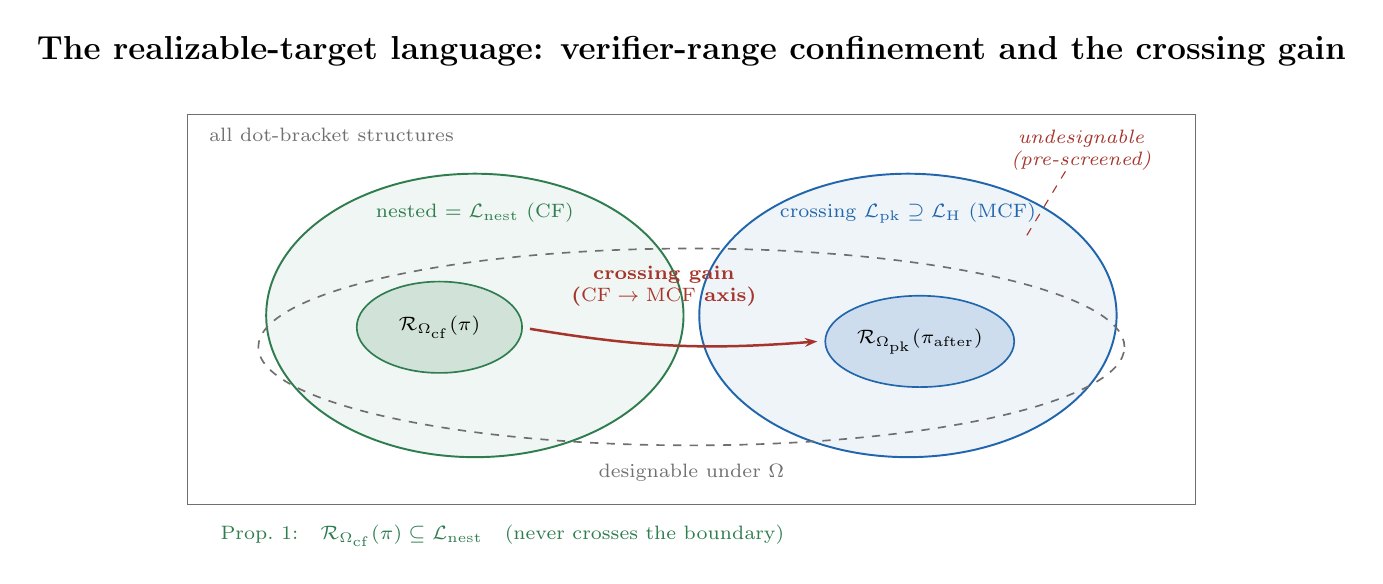
\begin{tikzpicture}[>={Stealth[length=4.5pt,width=3.2pt]}, font=\footnotesize]
\node[font=\large\bfseries] at (0,3.4) {The realizable-target language: verifier-range confinement and the crossing gain};
\draw[greyc, line width=0.5pt] (-6.4,-2.35) rectangle (6.4,2.6);
\node[greyc, font=\scriptsize, anchor=west] at (-6.25,2.35) {all dot-bracket structures};
\draw[cfg, line width=0.7pt, fill=cfg!7] (-2.75,0.05) ellipse (2.65 and 1.8);
\draw[mcfb, line width=0.7pt, fill=mcfb!7] (2.75,0.05) ellipse (2.65 and 1.8);
\node[cfg, font=\scriptsize] at (-2.75,1.35) {nested $=\mathcal{L}_{\mathrm{nest}}$ (CF)};
\node[mcfb, font=\scriptsize] at (2.75,1.35) {crossing $\mathcal{L}_{\mathrm{pk}}\supseteq\mathcal{L}_{\mathrm H}$ (MCF)};
\draw[greyc, line width=0.6pt, dashed] (0,-0.35) ellipse (5.5 and 1.25);
\node[greyc, font=\scriptsize] at (0,-1.95) {designable under $\Omega$};
\draw[cfg, line width=0.6pt, fill=cfg!22] (-3.2,-0.1) ellipse (1.05 and 0.58);
\node[font=\scriptsize] at (-3.2,-0.1) {$\mathcal{R}_{\Omega_{\mathrm{cf}}}(\pi)$};
\draw[mcfb, line width=0.6pt, fill=mcfb!22] (2.9,-0.28) ellipse (1.2 and 0.58);
\node[font=\scriptsize] at (2.9,-0.28) {$\mathcal{R}_{\Omega_{\mathrm{pk}}}(\pi_{\mathrm{after}})$};
\draw[->, negr, line width=0.9pt] (-2.05,-0.12) to[bend right=7] (1.6,-0.28);
\node[negr, font=\scriptsize\bfseries, align=center] at (-0.35,0.42) {crossing gain\\($\mathrm{CF}\rightarrow\mathrm{MCF}$ axis)};
\node[negr, font=\scriptsize\itshape, align=center] at (4.95,2.15) {undesignable\\(pre-screened)};
\draw[negr, line width=0.4pt, dashed] (4.75,1.88) -- (4.25,1.05);
\node[cfg, font=\scriptsize] at (-2.4,-2.75) {Prop.~1:\quad $\mathcal{R}_{\Omega_{\mathrm{cf}}}(\pi)\subseteq\mathcal{L}_{\mathrm{nest}}$\quad (never crosses the boundary)};
\end{tikzpicture}
\end{document}
